\documentclass[fleqn]{article}

\usepackage[utf8]{inputenc}
\usepackage[russian]{babel}
\usepackage{fullpage}
\usepackage{graphicx}
\usepackage{amsmath}
\usepackage{amsmath,amssymb}
\usepackage{mathbbol}
\usepackage{chngcntr}
\usepackage{hyperref}
\DeclareMathOperator{\E}{\mathbb{E}}
\DeclareMathOperator{\V}{\mathbb{Var}}
\DeclareMathOperator{\B}{\mathbb{Bias}}
\counterwithin*{equation}{subsection}
\counterwithin*{equation}{section}

\newcommand\independent{\protect\mathpalette{\protect\independenT}{\perp}}
\def\define#1{\textbf{def} \textbf{#1}}
\def\independenT#1#2{\mathrel{\rlap{$#1#2$}\mkern2mu{#1#2}}}

\DeclareMathOperator*{\argmin}{argmin} % no space, limits underneath in displays
\DeclareMathOperator*{\argmax}{argmax} % no space, limits underneath in displays

\begin{document}

\section*{Интро}
Заметки по ходу чтения книги Judea Pearl "Causality models, reasoning and inference".

\section*{A Theory of Inferred Causation}

\subsection*{Интуиция}
Начнем с интуиции, которая стоит за причинно-следственными связями. Обычно необходимым условияем является временная зависимость - причина происходит до следствия. Однако, очевидно, это далеко не всегда является достаточным условием для наличия причинной связи, поэтому остается вопрос, же ее установить?

Возможно ли в целом какое-то выявление причинно-следственных связей? На самом деле, да. Рассмотрим пример, где есть три события $A, B, C$ и мы знаем, что $A$ зависимо с $B$, $B$ зависимо с $C$, но $A$ и $C$ независимы. В таком случае, если немного подумать, выходит, что наиболее простой граф, описывающий такую конфигурацию, выглядит как на \ref{fig:abc}


\begin{figure}[h]
	\begin{center}
	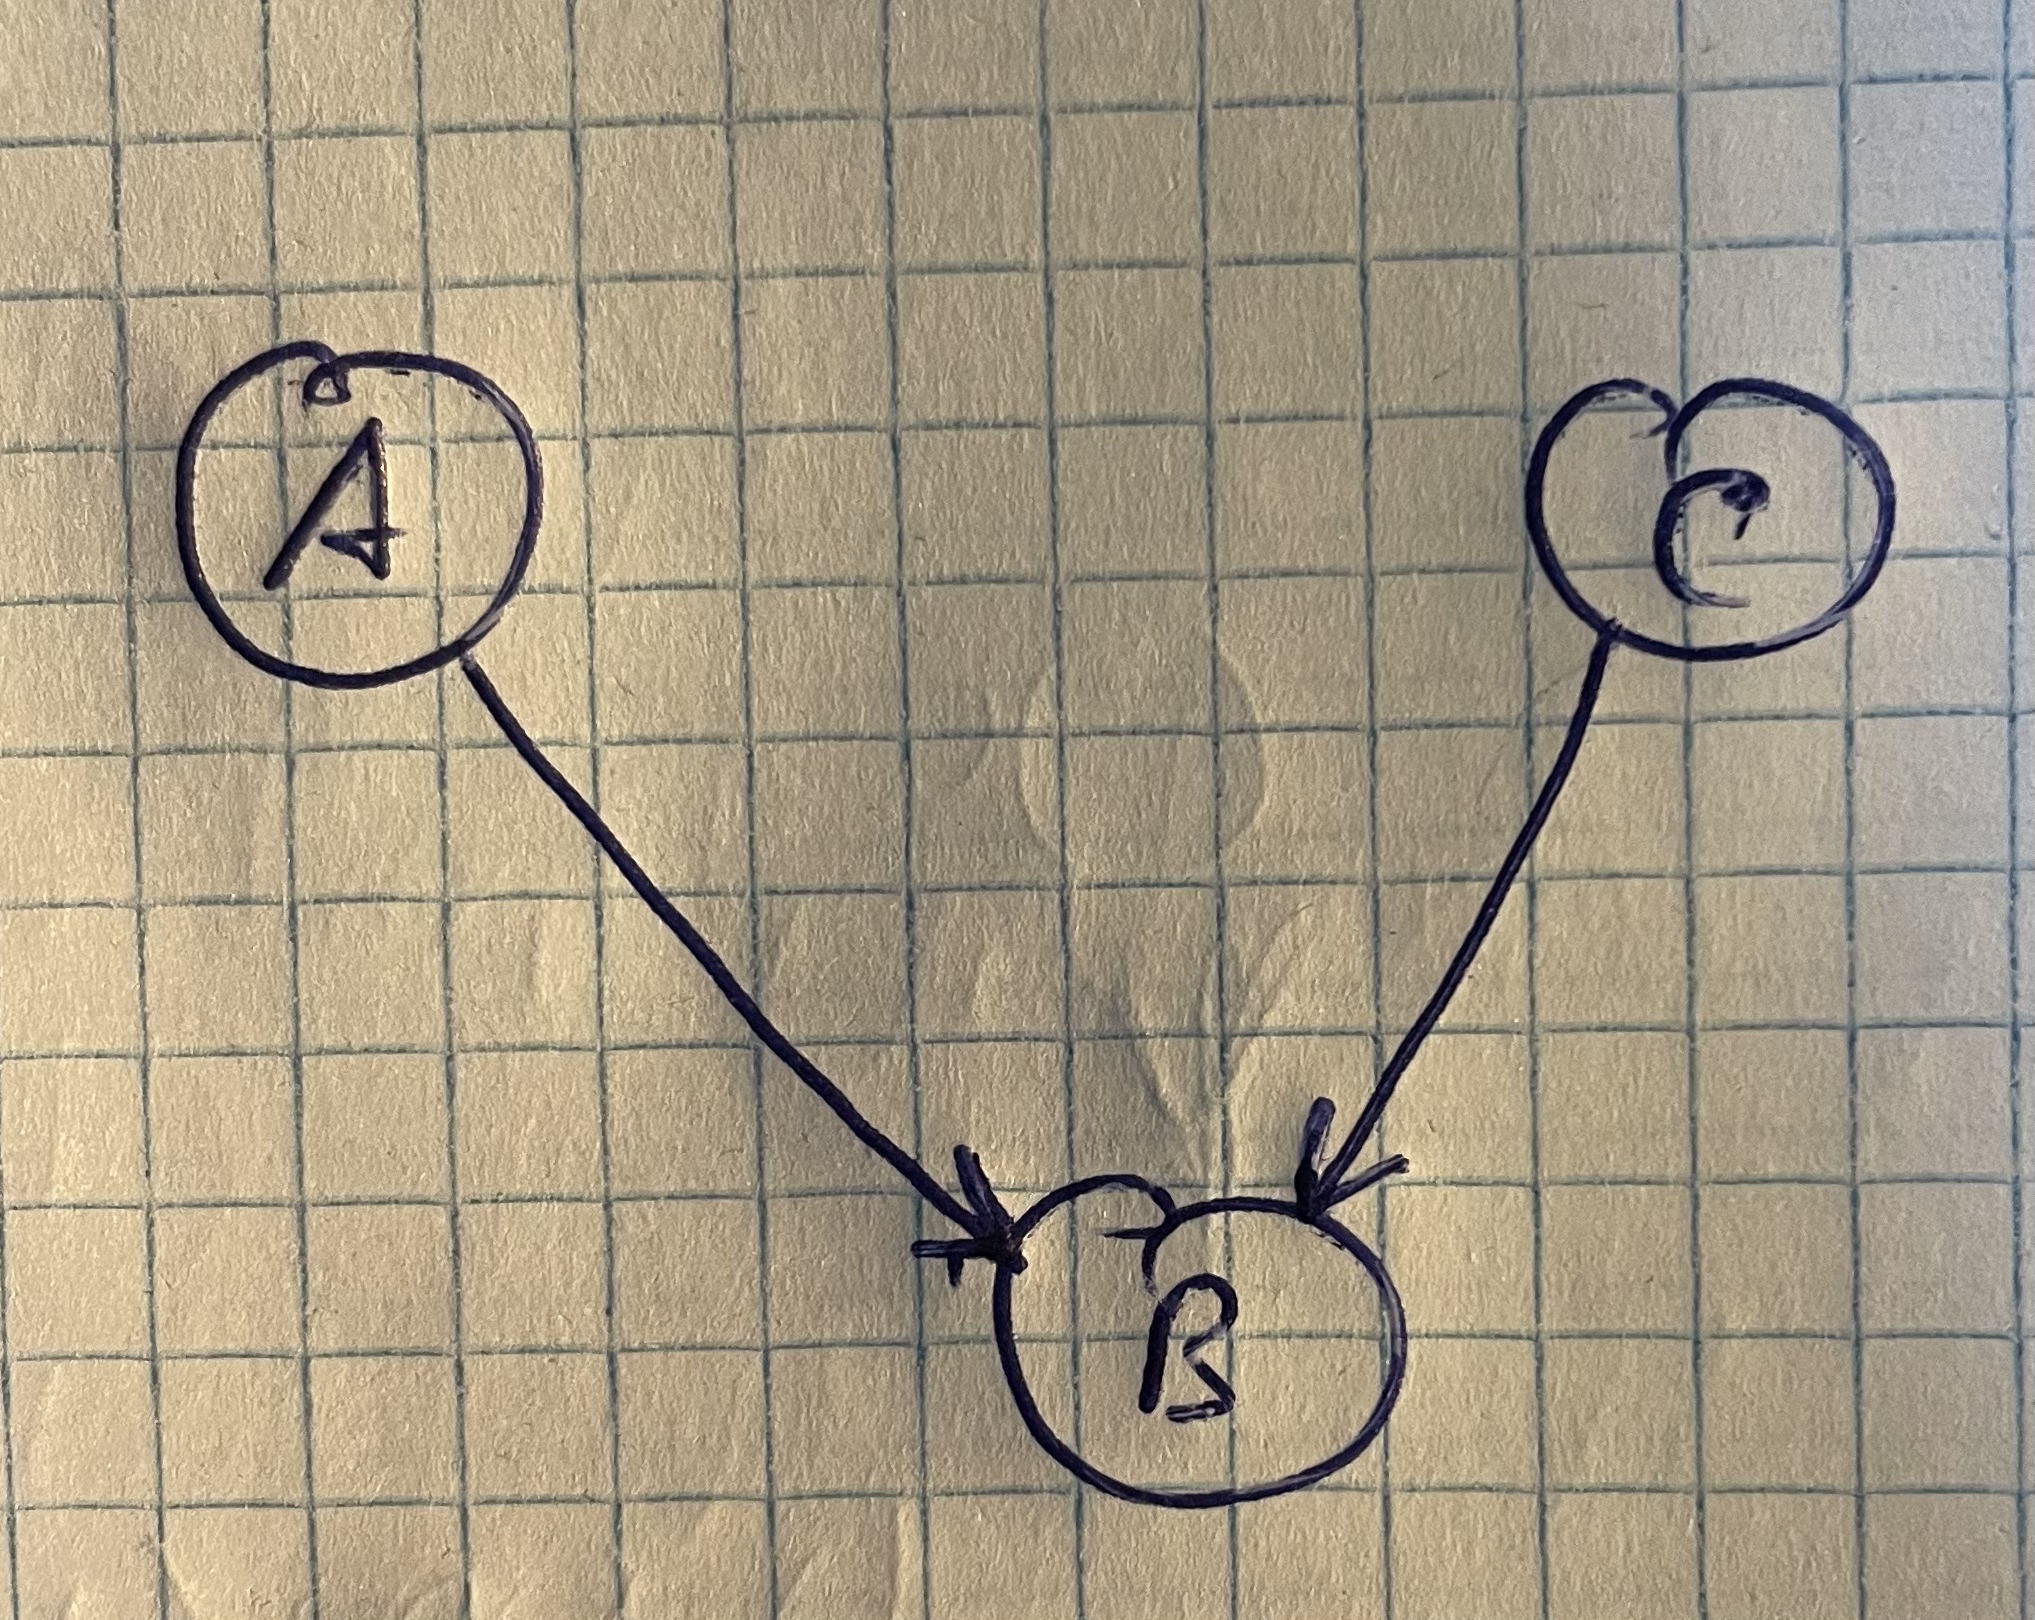
\includegraphics[scale=0.1]{imgs/img1.png}
	\end{center}
	\caption{A, C безусловно независимы, но зависимы при наблюдаемом следствии B}
	\label{fig:abc}
\end{figure}

Будем рассматривать задачу определения причинно-следственных связей в виде индукционной игры (индукционность в смысле что про некоторым примерам выводится какое-то общее парвило), в которую ученый играет с природой (красивая формулировка конечно XD). предполагается, что у природы есть стабильные причинно-следственные механизмы, которые можно определить функциональными зависимостями между переменными, некоторые из которых впрочем ненаблюдаемы.


\subsection*{Фреймворк}

\define{Причинная структура (causal structure)} множества переменных $V$ - это DAG, в котором вершинам соответствуют переменные, а рёбрам - прямая функциональная зависимость между соответствующими перемнными.

Причинная структура - это грубо говоря макет для \textbf{причинной модели} - точного определения того, как одни переменные влияют на другие.

\define{Причинная модель (causal model)}  - пара $(D, \Theta_D)$ из причинной структуры $D$ и множества параметров $\Theta_D$, ей соответствующих, то есть описывающих конкретные функциональные зависимости между переменными $V$ в виде $x_i = f_i(pa_i, u_i)$ $\forall x_i \in V$, где $PA_i$ - родители $x_i$ согласно $D$, $U_i$ - случайный шум, вероятностное распределение над которым также определяется $\Theta_D$.

Шум, влияющий на значение переменных, можно рассматривать например как следствие ненаблюдаемости некоторых переменных, и считается взаимонезависимым: ($U_i \independent U_j$).

Теперь задачу, поставленную перед гипотетчисеким учёным, можно сформулировать в виде восстановления причинной структуры, а затем и модели, при условии что он наблюдает лишь значения некоторого подмножества переменных $O \subset V$.

\subsection*{Выбор модели}

Вообще говоря, так как $V$ неизвестно, можно придумать сколь угодно много разных моделей, которые смогу зафитить данное (эмпирически определённое) распределение $P(O)$, путём различного введение скрытых переменных. Например, можно ввести одну скрытую переменную $U$, которая будет причиной всех наблюдаемых переменных $O$, при этом никаких причинно-следственных связей между наблюдамемыми переменными в такой модели не будет, причинная структура для такой модели представлена на \ref{fig:useless_model}.

\begin{figure}[h]
	\begin{center}
		\includegraphics[scale=0.1]{imgs/img2.png}
	\end{center}
	\caption{Довольно бесполезная причинная структура}
	\label{fig:useless_model}
\end{figure}

Идея выбора модели состоит в том, чтобы в некотором смысле она была наиболее простой/минимальной относительно тех данных, которые наблюдаемы.

Дальше введем не совсем формальное пока-что определение выведенной причинности (пока полагаем, что все переменные наблюдаемые)

\define{Выведенная причинность (предв.)} Переменная $X$ имеет причинное влияние на переменную $Y$, если существует направленный путь из $X$ в $Y$ в любом минимальной \textbf{причинной} структуре.

\define{Скрытая структура (latent structure)} это пара $L = (D, O)$, где $D$ - причинная структура над $V$, $O \subset V$ - множество наблюдаемых переменных.

\define{Предпочтение структуры (structure preference)} структура $L = (D, O)$ предпочтительнее структуры $L' = (D', O')$ (пишут $L \preceq L'$) если $D'$ эквивалентно $D$ на множестве наблюдаемых переменных $O$, т.е. тогда и только тогда, когда  $\forall \Theta_D \  \exists \Theta_{D'} : P_{[O]}((D', \Theta_{D'})) = P_{[O]}((D, \Theta_{D}))$. 

Латентные структуры называются эквивалентными, если $L \preceq L'$ и $L' \preceq L$. 

\define{Минимальность (minimality)} структуры $L$ относительно класса структур $C$ означает её предпочтительность относительно всех других структур этого класса: $\forall L' \in C \ L \preceq L'$.

\define{Согласованность} латентной структуры $L = (D, O)$ с распределением $\hat P$ над $O$ означает возможность разместить $\hat P$ в данной латентной структуре, то есть что $\exists \Theta_D : P((O, \Theta_D)) = \hat P$.


\define{Выведенная причинность} С данной $\hat P$ над $O$, переменная $X$ имеет причинное влияние на переменную $Y$, если существует направленный путь из $X$ в $Y$ в любой минимальной \textbf{латентной} структуре.

Надо отметить, что экспрессивная мощность латентной структуры тем выше, чем меньше в ней закодировано независимостей между переменными: таким образом, структуры с меньшим числом незавимостей, согласованные с данными, будут менее предпочтительны, чем структуры с большим числом независимостей в причинной структуре.

\subsection*{Стабильные распределения}

Концепция минимальности латентной структуры позволяет корректно и непротиворечиво получать выводы о причинных связях переменных. Однако, это не всегда вычислительно просто - различных конфигураций структур может быть очень много, и проверять каждую из них на минимальность может быть очень дорого. К тому же, вообще говоря, может же оказаться, что настоящий процесс, генерировавший данные, все таки был порожден моделью, отличной от минимальной? Чтобы упростить себе жизнь, предлагается ввести в рассмотрение ещё один принцип, помимо минимальности - принцип стабильности. 

Начнем с небольшого примера. Рассмотрим процесс, в котором есть две честные монетки. Множеством событий будет выпадение монетки $A$, выпадение монетки $B$, и событие $C$ - "монетки выпали одинаковой стороной". нетрудно заметить, что любая пара переменных безусловно независима, но зависима при условии третьей переменной (например, $P(A=1) = P(A=1|B) = 0.5\ \forall B$, но $P(A=1|B=1) =0.5\neq P(A=1|C=1,B=1) = 1$). Таким образом, любая из структур на \ref{fig:choice} допустима с точки зрения данных и является минимальной. В то же время, если чуть пошатать параметры распределения, например сделать $P(A=1) = 0.6, P(A=0)=0.4$, то уже однозначно не подойдет структура, где $C$ и $B$ независимы безусловно, так как будет $P(C=1) = 0.5$, но $P(C=1|B=1) = 0.6$. Аналогично можно пошатать вероятности для второй монетки, сделав её не совсем честной, и отбросить модель, где $A$ и $C$ независимы.

\begin{figure}[h]
	\begin{center}
		\includegraphics[scale=0.07]{imgs/img3.png}
	\end{center}
	\caption{Какую из трех причинных структур выбрать?}
	\label{fig:choice}
\end{figure}

Для того, чтобы разрулить такие неоднозначности, вводится понятие стабильности:

\define{Стабильность (распределения)} Пусть $I(P)$ - множество всех независимых отношений переменных, заданных через $P$. Причинная модель $M = (D, \Theta_D)$ генерирует стабильное распределение тогда и толкьо тогда когда в $P((D, \Theta_D))$ нет никаких лишних независимостей, т.е. $I(P((D, \Theta_D))) \subset I(P(D, \Theta_{D'}))\ \forall \Theta_{D'}$.

По смыслу, при варьировании параметров от $\Theta$ к $\Theta'$ никакие независимости не должны рушиться, если распределение стабильно. Что пока непонятно - а как выбирать, какие из вероятностей шатать: видимо те которые не ноль? Тогда и правда из стабильности остается только один вариант из трех в приведенном выше примере.

\subsection*{Реконструкция причинной структуры (DAG)}

\end{document}